%%%%%%%%%%%%%%%%%%%%%%%%%%%%%%%%%%%%%%%%%%%%%%%%%%%%%%%%%%%%%%%%%%
%  = PREAMBLE =
% The preamble of a LaTeX document is the set of commands that 
%    precede the \begin{document} line.  It sets up the style of 
%    the document.
%%%%%%%%%%%%%%%%%%%%%%%%%%%%%%%%%%%%%%%%%%%%%%%%%%%%%%%%%%%%%%%%%%

\documentclass[aps,twocolumn, secnumarabic,balancelastpage,amsmath,amssymb,nofootinbib,floatfix]{revtex4-1}

\usepackage{graphicx}      % tools for importing graphics
\usepackage[colorlinks=true]{hyperref}  % this package should be added after 
\usepackage{parskip}
                                        % all others.
                                        % usage: \url{http://web.mit.edu/8.13}


%%%%%%%%%%%%%%%%%%%%%%%%%%%%%%%%%%%%%%%%%%%%%%%%%%%%%%%%%%%%%%%%%%%
% And now, begin the document...
%%%%%%%%%%%%%%%%%%%%%%%%%%%%%%%%%%%%%%%%%%%%%%%%%%%%%%%%%%%%%%%%%%%

\begin{document}

\title{Response to Homework 2}
\author{Yongao Hu}
\email{yongao@mit.edu}
\date{\today}
\affiliation{MIT Department of Physics}


\begin{abstract}
The following graph presents the aggregate data of gravitational acceleration $g$. The data is collected from all the students across the years. The result is $g = (9.84 \pm 0.61)$ m/s$^2$. The error is the standard deviation of the data. The result is consistent with the known value of $9.80$ m/s$^2$.
\end{abstract}

\maketitle

\begin{figure}[hbt!]
    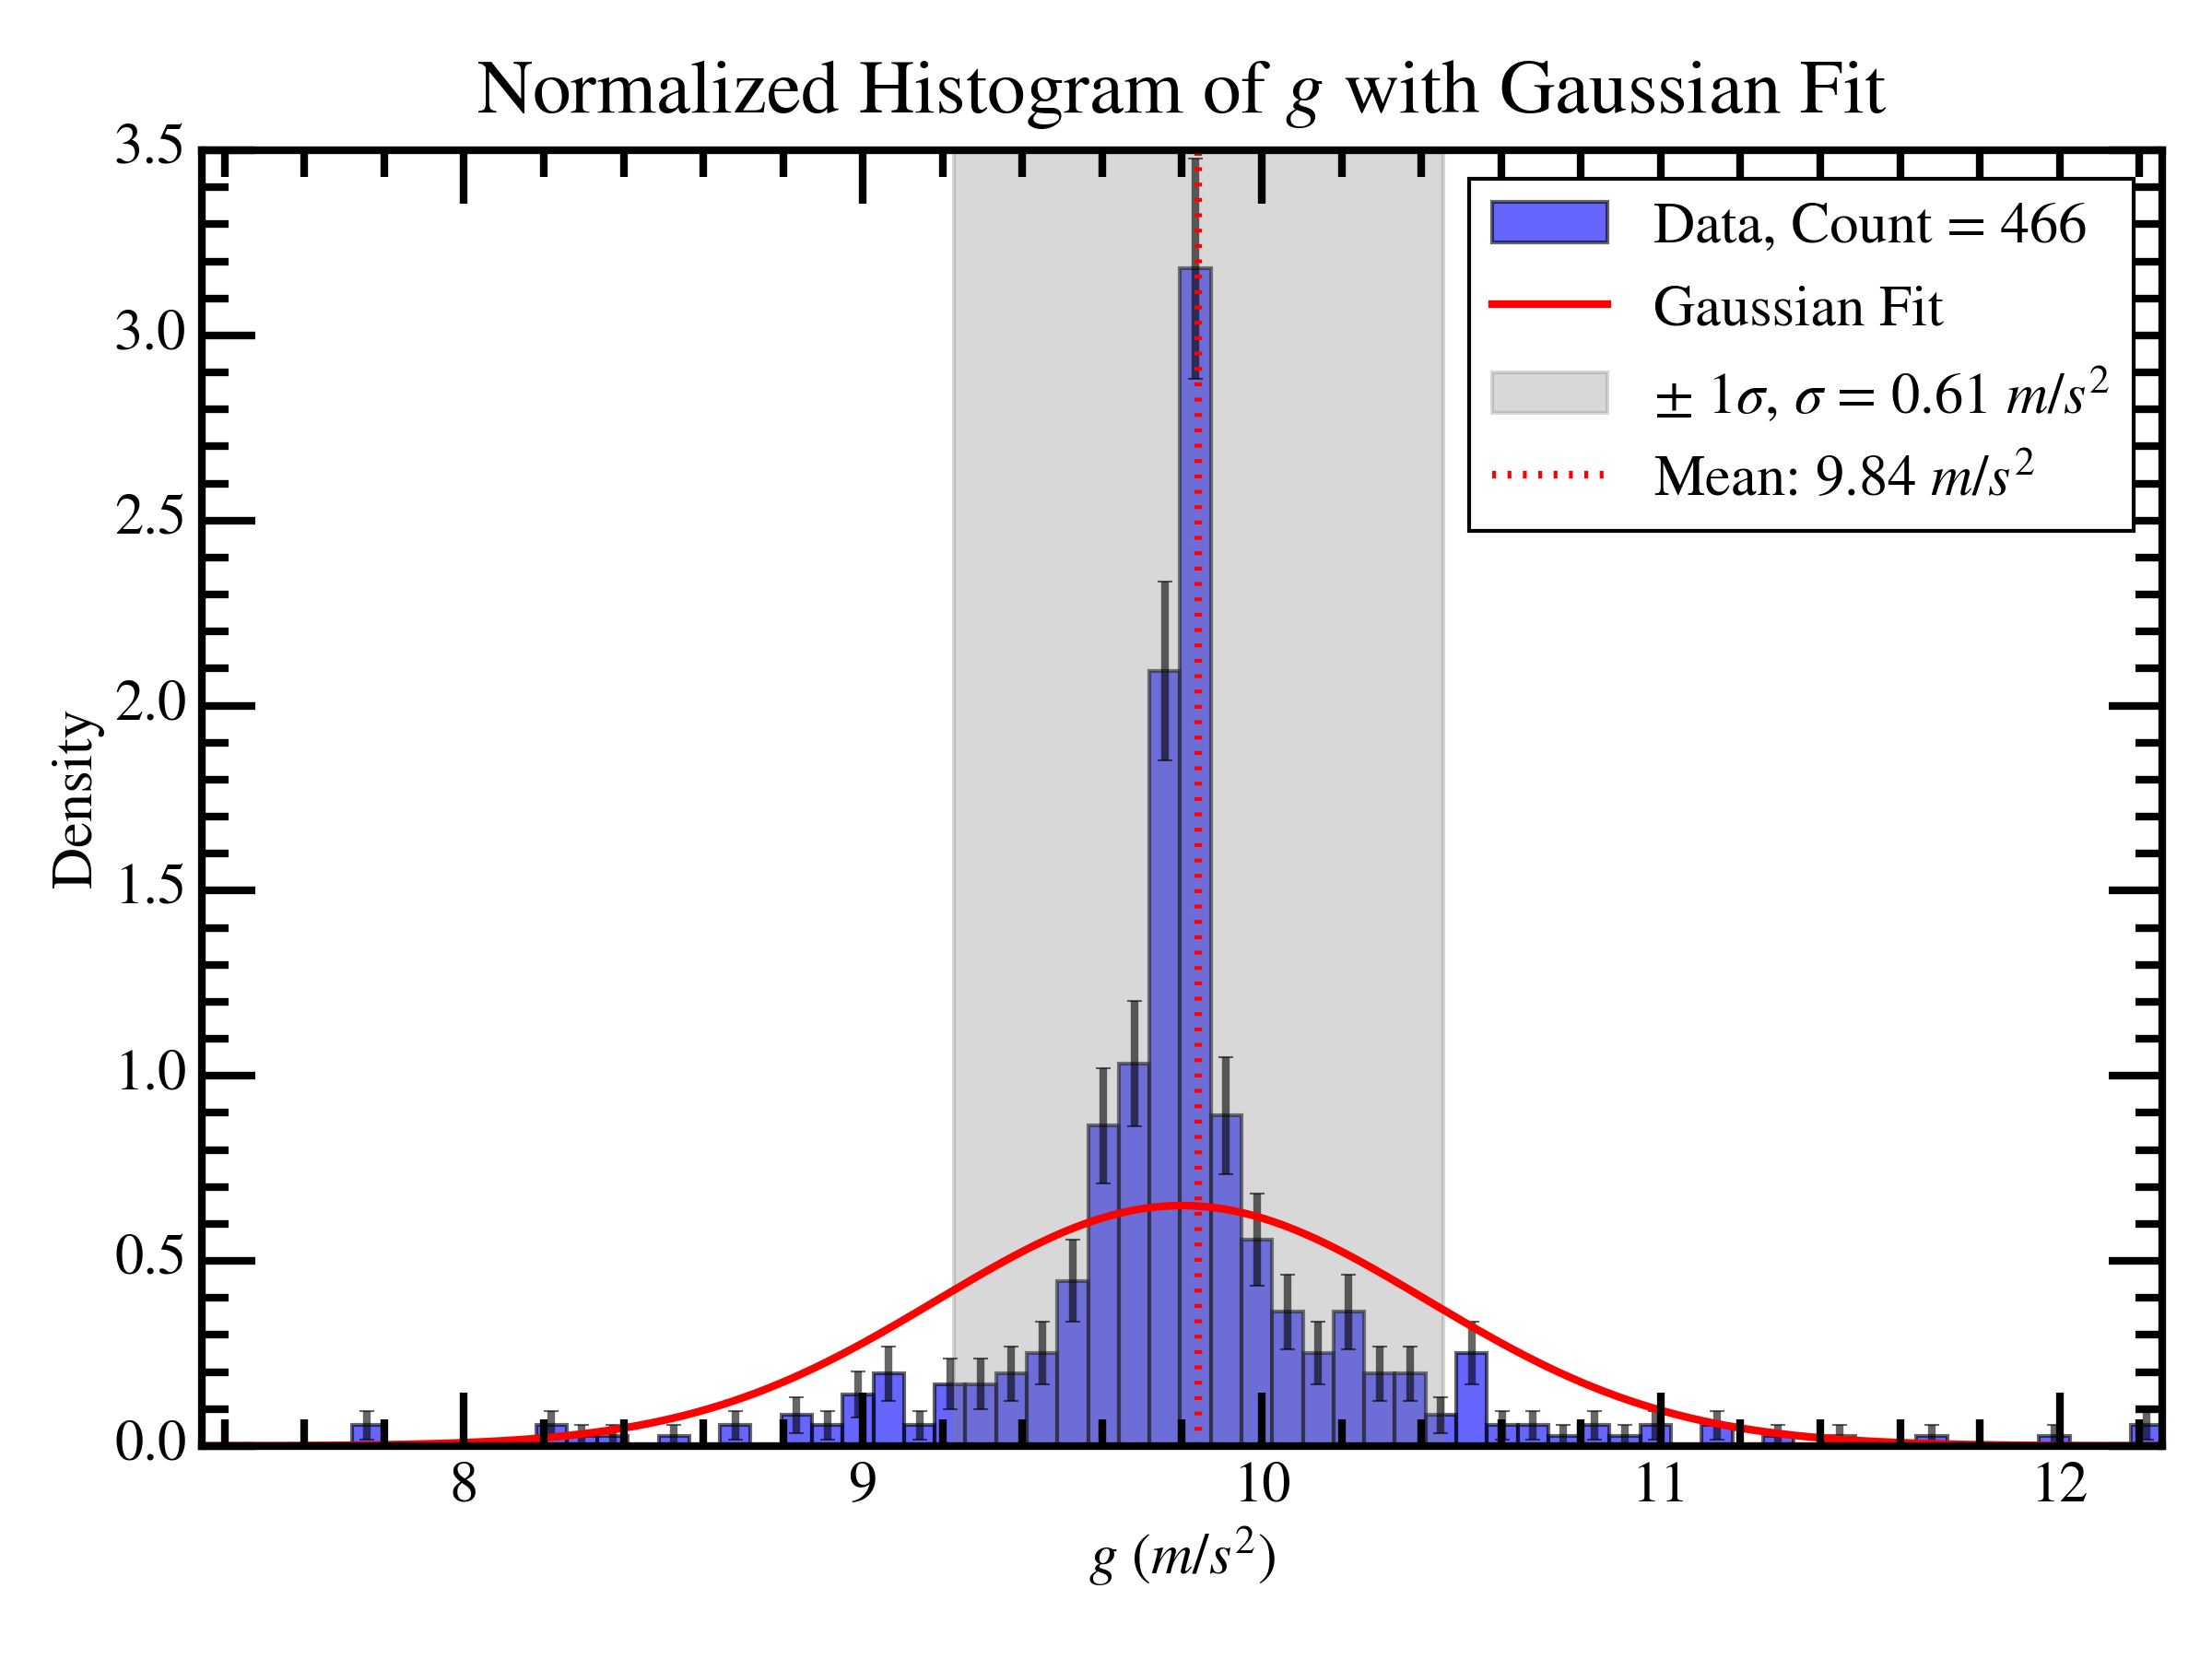
\includegraphics[width = 0.8\linewidth]{PendulumDataHistogram.png}
    \caption{Histogram of the gravitational acceleration $g$ measured by students. The result is $g = (9.84 \pm 0.61)$ m/s$^2$. The error bar is the poisson error; the aggregate uncertainty is the standard deviation of the data.}
\end{figure}


\begin{acknowledgments} The author gratefully acknowledges their lab partner V. Tran for their invaluable help in the plots described here.
\end{acknowledgments}




\bibliography{simple-paper}

\end{document}

